
\subsection{Research Field Classification}
\label{sec:field_classification}
\subsubsection{Task Description}
The goal of this task is to identify the research fields covered in the social science publications.
In general, two approaches could be applied to this task.
One is the extraction of relevant terms of the publications.
It means that this task could be seen as a keyword extraction task and the detected terms considered as descriptive terms regarding the research field.
The second approach is to learn to classify publications research fields with the use of annotated data in a superviesed manner.
The benifit of the second approach is that the classification scheme to describe the research field can be defined experts of the domain.
The disadvantage of supervised trained classifiers for this task is the lack of applicable training data.
Furthermore, it must be ensured that the training data is comparable to the texts the research field classifier should be applied on.

%% * Formal definition
\paragraph{Formal problem definition}
Let $P$ denote a set of Publications of size $n$, $A$ a set of corresponding abstracts of the same size and $L$ a set of $k$ defined class labels describing research fields.
The task of research field classification is to select for each publication $p_i\in{P}$ based on the information contained in the corresponding abstract $a_i\in{A}$ a set of labels $C_i = \varnothing \cap \{c_1\dots c_n|c_n \in L\}$ of $n$ labels.
The number of $n$ denotes the number of labels from $L$ describing the research field of $a_i$ and can vary for each publication $p_i$.
If there is no label $l_k$ representing the information given by the abstract $a_i$ the set of class labels is the empty set $\varnothing$.


%\subsubsection{Challenges}
%% * Decision for Supervised
%%  * No Gold standard given
%%  * Known Corpus from similar domain
%%  * benefits of SSOAR corpus
%%  * Why is it good
%%  * Because of courpus we decided to go for a supervied method

\subsubsection{Our approach - Overview}
%% External data (SSOAR
%% * Supervised
%% * Multi label classification
Since we didn't receive any gold standard for this task during the competition we decided to make use of external resources.
We decided to use an external labeled dataset to train a text classifier which is able to predict for a given abstract of a publication one or more research field label.

The publications given througout the competition belongs to the domain of social sciences we considered metadata from a open access repository for the social sciences called SSOAR.
The advantages are twofold.
On the ond hand, we could rely on professional annotations in a given classification scheme covering the social sciences and related areas.
On the other hand the source is openly available.\footnote{A script to download the metadata of SSOAR can be found in github/research-field-classifier}

%% * Classification schmeme Classoz (Why it seems usefull)
The annotated data of SSOAR contains four different annotation schemes for research field related information. By reviewing these schemes, We decided to use the Classification Social Science (classoz) annotation scheme. The number of classes in each schema, coverage of each classification, and the distribution of data in each schema affected our decision. 
An exhausitve description of the used data can be found in \ref{sec:external_data_sources}.

%% * data pre pro
\paragraph{Pre-processing and model architecture}
%%  * selected fields and language
%%  * titles are often german
SSOAR is a multilingual repository.
Also the available abstracts can vary in language which can differ to the language of the publication.
We selected all English abstract with valid classification as our dataset.
Mainly because of the language of the RCC corpus.
But it has to be noted, that the multilingual SSOAR-abstract-corpus has a skewed distribution of languages with English and German as the main languages.
We count 22,453 English abstracts with valid classification after filtering.
%%  * skipped label
Due to the unequal distribution of labels in the dataset, we need to guaranty enough training data for each label.
We selected only labels with frequency over 300 for training the model, which results in a total of 44 out of 154 classification labels representing research fields.
%%  * Train test split
For creating train and test set, 22,453 SSOAR publications with their assigned labels were split randomly.
We used a train/validation/test split of 70/10/20.
%%* Our model
We decided to train a text classifier based on the fasttext framework~\cite{joulin2017bag}.
The arguments to use this model was the speed in comparison to a more complex neural net archiecture and the still comparable to state of the art performance (e.g.\cite{wang2018joint}).
%%  General used Fasttext parameter
The model is trained with learning rate 1.0 for 150 epochs.
Also, the negative sampling parameter is set to 25.


\subsubsection{Evaluation}
%% metrics
%%  preci recal f1 micro
%%  ...
%% Parameter Selection
%%  k and threshold
%%  * reduced number of labels?
In this experiment, only the top 3 labels with the highest probabilities were considered for the evaluations.
Figure~\ref{fig:fields_precision_recall} shows the performance of the model regarding various evaluation metrics for different thresholds.
A label is assigned to a publication if the model outputs a probability for the label above the defined threshold.
In multi-label classification, this allows us to evaluate our model from different perspectives. 
As it is illustrated in figure~\ref{fig:fields_precision_recall}, the point that the micro-precision curve and micro recall meet is at the threshold of 0.1.
%% final results
We can see the point as the highest point of micro f1-measure. By increasing the threshold from this point, the micro-precision score is increasing, but the micro recall is falling. By Decreasing threshold, these trends are opposite.  Also, the default threshold doesn't look promising. In spite of micro-precision about 0.7, we have a problem with the very high number of items without any prediction. 
%%  comparison to baseline (SVM?)

%%\subsubsection{Discussion}
%%  What do the results show
%%    For how many samples of the test set do we have prediction
%%    How well is the classifier performing on given classes
%%    Performance on different data can not be measure
%%      results from rcc judges are promissing
%%    Lack of generelizability (domain)



%The x-a  the change of  metrics over different probability thresholds for generating the result.
\begin{comment}

This graph shows the change of different evaluation metrics over different probability thresholds for generating the result. 
The threshold defines the minimum probability of a label which is leading to an assignment.

Orderly, micro precision and micro recall values are 0.5 for threshold 0.1
For this threshold, the model generates a prediction for all items and about half of the items have at least one correct prediction. 
All these metrics remain the same till threshold 0.2. Till threshold 0.6, we can see a dramatic increase in the micro precision and the number of items without any correct prediction. Both of these metrics pass 0.8. On the other hand, micro recall falls to the below of 0.2. In this case, selecting threshold seems hard task, since the conflict point of precision and recall is a threshold about 0.25 but both of these metrics at the point are not more than 0.3 and also we have more than 0.4 items with completely wrong predictions. Also, the default threshold doesn't look promising. In spite of micro precision about 0.7, we have a problem with the very high number of items without any prediction.
\end{comment}

\begin{figure}[t]
\centering
%\subfloat[Random Forest Evaluation]{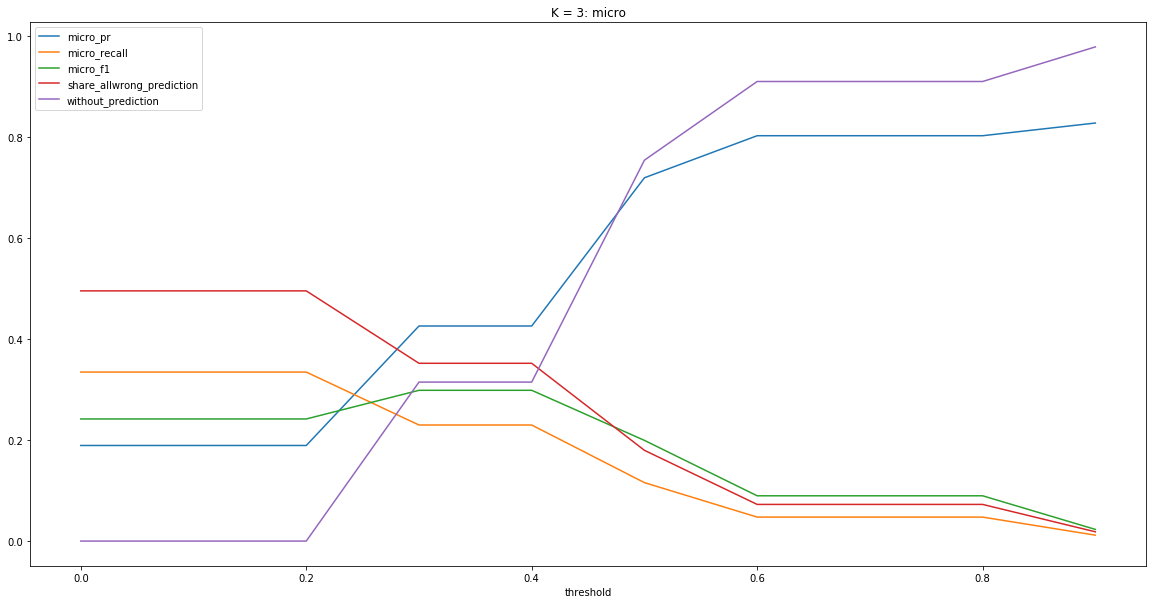
\includegraphics[width=0.49\textwidth]{figures/research-fields/random-forest-evaluation.png}\label{fig:rf}}
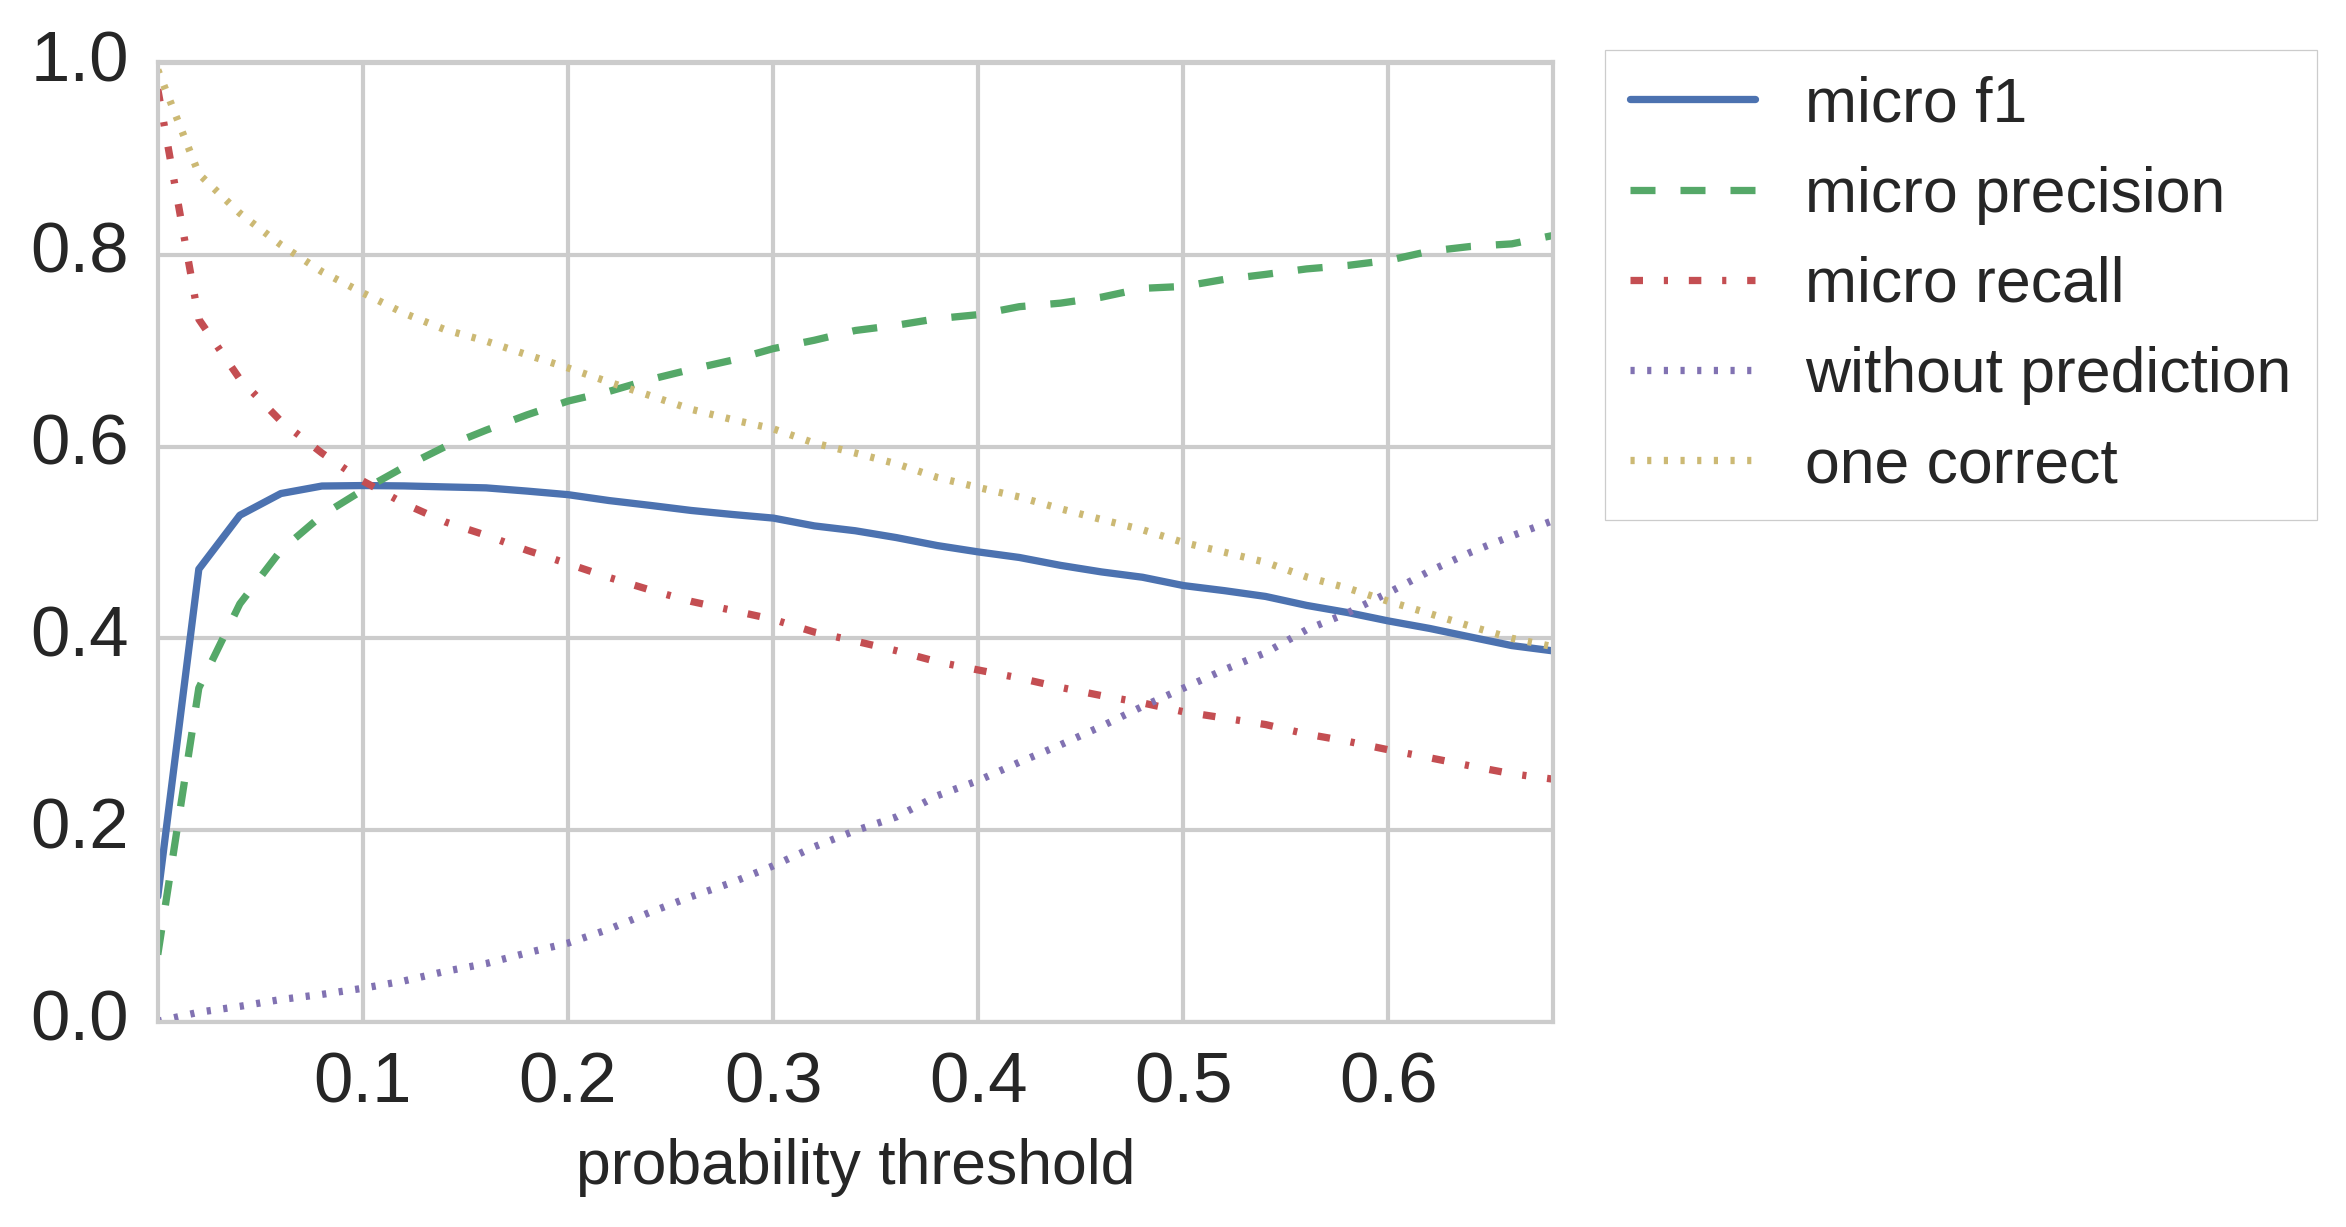
\includegraphics[width=.49\textwidth]{figures/research-fields/fields-precision-recall.png}
%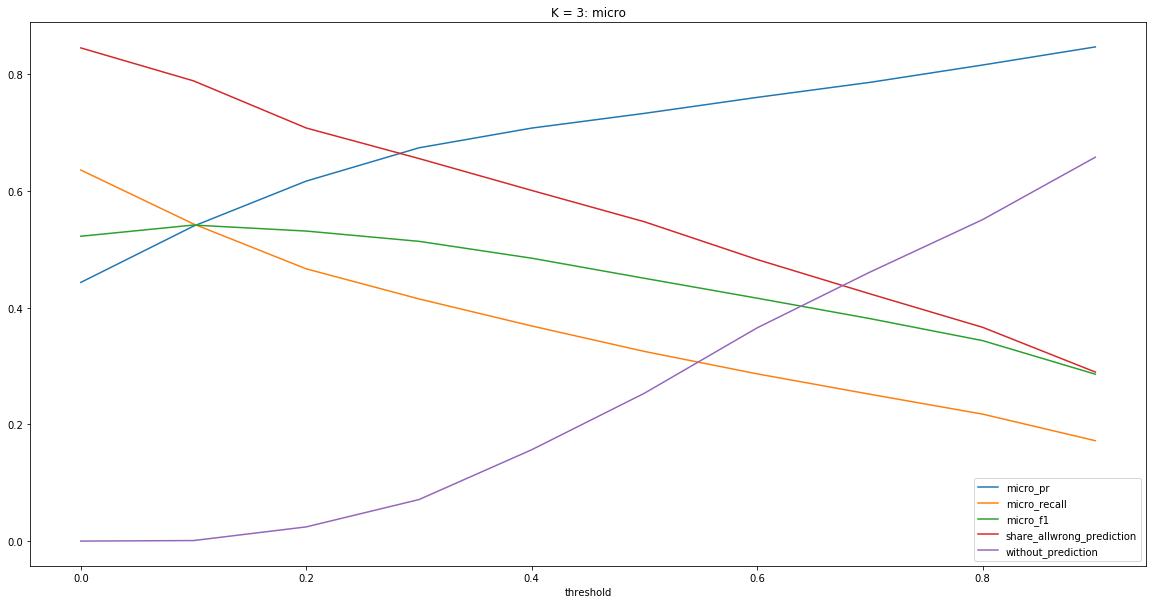
\includegraphics[width=.49\textwidth]{figures/research-fields/fast-text-evaluation.png}
%\vspace{-1em}
    \caption{Metrics for different selected probability thresholds (validation set)}
\label{fig:fields_precision_recall}
\end{figure}


\begin{table}[b]
\center
\small
    \caption{Evaluation results on test set (Fasttext model)}
  \label{tab:eval_research_field}
  \begin{tabular}{ll}
  \toprule
      Metric & Value \\
  \midrule
      Micro F1:          & 0.529 \\
      Micro Precisison:  & 0.499 \\
      Micro Recall: 	 & 0.564 \\
  \bottomrule
\end{tabular}
\end{table}

%The trends of micro f1, micro recall, and publications with just wrong predictions are falling smoothly, but the trend of micro precision and number of publications without any prediction are rising gradually. 
%The Micro precision still is higher than 0.7 for threshold 0.4. Also, the number of items without prediction is lower in threshold 0.4 than threshold 0.5 (the difference is about 0.1).

% We also experiment with random forest 



%purple curve (without_prediciton) 
%The measure without_prediction describes the share of publications without any prediction at all.
%E.g. if we only accept predicted labels with a model certainty of 60\%, 40\% of the publication have no predictions. 

%red curve (share_allwrong_prediction)
%The red curve describes the share of documents in the test set, which contain only wrong predictions for each threshold.
%This means when a threshold of 20\% certainty is selected 70\% of the publications have only wrong predictions. But if a threshold of 80\% certainty is selected only 40\% of the publications have only wrong predictions. 
